\documentclass[a4paper]{scrartcl}
\usepackage{apacite}
\usepackage[english]{babel}
\usepackage[utf8]{inputenc}
\usepackage{amsmath}
\usepackage{graphicx}
\usepackage[parfill]{parskip}
\usepackage{todonotes}
\usepackage{csquotes}
\usepackage{tabularx}
\title{Master's thesis proposal II}
\author{Stijn Voss, s4150511 }
\date{March 2017}
\begin{document}

\maketitle

\section{Introduction}
In the first part of my thesis proposal I considered using photo recognition to improve usability of food journaling. My main goal however is not to improve food journaling per se, but to build something that can actually help people eat healthier. My main philosophy here is that this should be done in a iterative fashion. First start with something small, that works well enough to reach a significant amount of users. The resulting resources, lessons and data can then be used to further improve and extend your approach while at the same time technology advances. 

Especially I belief that data might help dealing with the behavioral sciences part of eating healthy. For example while calorie intake might be the most important factor for a healthy weight. Different types of diets might actually make eating less calories more or less difficult: If you eat the same amount of sugar or vegetables in terms of calories, vegetables will probably make you feel more satisfied. Certain factors like stress or social factors might also play a role. When you want to test this in an controlled environment this is likely to be difficult: the fact that an subject is participating in a experiment, will influence it's behavior. Together with the huge quantities of data you can collect using such an application I believe that you might eventually find some very interesting insights and solutions. 

So my first idea was to see if I could improve food journaling significantly by using photo recognition. However I quickly found that this was more difficult than I thought at first. Mainly because there is no trivial way of categorizing food and not all the ingredients will be visible. I therefore proposed to do the best thing I could still do and think of: mapping all visible and relevant information into a invariant vector space, while filtering out the rest. 

However such a vector will probably always have to be used together with context in order to be useful. For example knowing what someone has bought, what someone has eaten before and where someone is(certain restaurant or at home?) Knowing what someone has bought however will be difficult in practice(working together with super markets would be interesting, but that's a difficult starting point). Photo recognition does not have a lot of advantages compared to choosing from meals by hand, when it comes to restaurants and meals eaten before. 

Another interesting type of input, next to photo recognition, is textual input of recipes and meals. I am mainly thinking of building a large web corpus of recipes and meals. This meal corpus can then be used to come up with suggestions based on search queries or maybe photo queries. Or even better propose healthier alternatives that people may like. To make this work we have to label our data with properties that users would like to query for: nutritional information, ingredients and preparation time for example. 

It could also allow users to plan their food intake ahead instead of only logging it at the moment of eating. Which they can use to make shopping lists for example. Using the web as a corpus also has the advantage that it becomes easier to deal with cultural differences. As long as there are recipes available for that country or culture on the web, we can gather relevant recipes. 


\section{What is a recipe?}
It might be valuable to think about what our data looks like: 
\begin{itemize}
\item \textbf{Title:} Almost all recipes will have a title
\item \textbf{Ingredients:} A list of ingredients in textual format. These ingredients very often also contain a quantity estimation in textual format. (Some sites will also provide these separately but for the generalization power of our method it might be beneficial to assume they are just in textual format). Like `250gr chicken breast`. To prevent confusion I will refer to `250gr' as the quantity, `chicken' as the ingredient and when I talk of the complete sentence(250gr chicken breast) I will talk about `ingredient sentence'.
\item \textbf{Recipe instructions:} A text describing how a meal has to be prepared  
\end{itemize}
Optionally these attributes could also be defined:
\begin{itemize}
\item \textbf{Image} often an image is attached displaying the meal
\item \textbf{Nutritional information}: Indicating the calories, proteins etc. present in the meal usually defined per serving but not necessarily
\item \textbf{Yield}: Indication of how much this recipe will make, usually defined in number of servings but not necessarily
\item \textbf{Prep, cook and total time}: The time the authors think it would take to cook and prepare the meal.
\item \textbf{Cuisine}: The cuisine of the meal: italian, american, french etc. 
\item \textbf{Restricted diets}: Vegetarian, paleo, low carb  etc.
\item \textbf{Category:} Breakfast, lunch, diner, appetizer etc. 
\end{itemize}
I based this on the schema.org recipe format\footnote{\url{http://schema.org/Recipe}}. But I assume that the authors had a look at the whole web before defining it, so I think its safe to assume that it is representative for the complete web. The schema.org structured dataset can best be described as a labeled textual dataset. The information it self is natural language with labels.  

As you can see most relevant information will already be available in the schema.org dataset i am planning on creating. However almost no attribute will be available for all recipes. Our basic task will be to learn these attributes for all recipes from the limited set that is defined. To do so we will have to deal with the vagueness of textual data.

As a consequence from the method I will propose I believe the following will also be simpler to solve:
\begin{itemize}
\item Learning nutritional information per ingredient sentence
\item Separating quantities from ingredient in ingredient sentences
\item `Understanding' textual quantity definitions and how they relate to one another
\item `Understanding' textual ingredient descriptions and how they relate to one another: vector space `brown rice` and `white rice` are very related. `Olive oil' and `bread' are less related. 
\item `Understanding' what ingredients sentences look like: which might be helpful if we want to index non schema.org websites. 
\end{itemize}
\section{Related work}
\todo[inline]{This section might a bit out of place, but this is where i started. }
One idea that I see used very often in other research is using vector spaces to deal with the very complicated nature of recipe data.   
\citeA{tansey2016diet2vec} wanted a way of analyzing all the data that LoseIt\footnote{\url{https://www.loseit.com/}} has of it's user. Users track their food intake by logging `food items'. Food items are user defined entries that are labeled with nutritional information. For example ingredients like rice or oil but also complete ready made meals. To deal with the enormous amount of data they apply word2vec on the food items to convert it to vectors. Then these vectors are combined with the attached nutritional info and clustered into 500 clusters using k-means. Next they combined the food vectors per meal usings paragraph2vec\cite{le2014distributed} and applied k-means again. Lastly they combined all the meals of a user using a similar approach and did the same. According to the authors the resulting clusters showed some clear diet patterns: like high protein diets or low protein diets etc.

Just representing the ingredients as vectors can also be useful. \citeA{food2vec} used 55.000 recipes and its ingredients and applied word2vec to convert them into vectors. Analogous to words in word2vec similar ingredients will be used with similar ingredients. However the ingredient lists of recipes are not sequential, they are unordered. The author therefore rightfully noted that predicting all other ingredients used by a given ingredient, using a multi-label classification technique like multi class logistic regression would make more sense. If you look at similar ingredients the vector space clearly shows some interesting properties, although it's definitely not perfect. One thing that the author notes is that more data would be valuable. Since you need quite some occurrences of each ingredient to make it work, especially if you consider synonyms. 
\section{Correlations to other natural language processing techniques}
\subsection{Ingredients can be interpreted as text or sentence}
One observation I made is that the quantities of the ingredients can also be seen as part of the recipe.  The quantities might actually be quite informative, depending on the exact task at hand. To predict the nutritional information of your recipe it is probably pretty important.  

Reading the ingredients could also be seen as reading a sentence or a piece of text. We could then let the algorithm figure out what part of the text is the quantity and what is the actual ingredient. Splitting the text into smaller pieces would make it possible for our algorithm to exhibit way more generalization power. For example it could learn that 1 tablespoon is a certain quantity estimation and that 2 tablespoons is twice as much. If it originally learned from the training data that 1 tbsp of ingredient x has y calories. It could possibly  learn that 2 tbsp of x has 2y calories, without having an exact example of this. \todo[inline]{Of course the network would have to be forced to actually learn this but since quantities are very important for nutritional information i would suspect that it happens when i make the number of parameters small enough}

For the ingredient it self their is also a lot to generalize, for example it can learn that the usage of the word `sliced' or a brand usually doesn't matter for the nutritional information. The fact that it already learned that `brown rice` and `Jasmin rice` have similar nutritional information, tells a lot about the nutritional value of `White rice`.

\subsection{Ingredients are to recipes what words are to sentences}


In general it seems that recipe data has a lot of similarities with natural language. Ingredient frequency distribution can usually be well described by a similar zip-Mandelbrot curve \cite{kinouchi2008non} for different cuisines. Where as for word frequency distributions for normal languages we usually see that these look like zipf-curves and are similar for different languages. We could thus also say that ingredients are to cuisines what words are to languages. Please note that this can be explained by similar  underlying development patterns that give rise to both cuisines and languages \cite{ahn2011flavor,dahui2005true} , but it might mean that similar models will work for this problem.

Also only a limited set of recipes is used compared to the theoretically number of recipes possible \citeA{ahn2011flavor}, which is probably also true for natural language. Where most sentences used will be only a fraction of the possible combinations. 
\todo{Maybe leave this out, not so precise}

\subsection{Related literature}
\subsubsection{Word embeddings}
\todo[inline]{Maybe explain word embeddings in the final thesis?}
\subsubsection{Word sequences}
In natural language processing tasks a very common task is to represent a sentence(or other sequences of words like paragraphs) as a vector. This is complicated since different sentences can have a different number of words. Early approaches would make use of the bag of words model. However in with this approach you will lose the value of word similarity(as also present in word embeddings) and the order of the words. If two sentences contain the words "Strong" and "powerful" respectively this an indication that they are close to if one of them would contain "Paris".

\citeA{le2014distributed} propose a method to make a vector of paragraphs that takes ordering and semantic similarity into account. They modify a CBOW word embedding model, where given the context(words around it) of a word the word has to be predicted, by also giving the paragraph id used. And similarly forcing this paragraph into a vector space. This way a vector space for the paragraphs is created. They also train a model where the task is to predict the words in a paragraph given by just the paragraph id it self. This way you would get a vector space for a paragraph that does take semantic similarity into account.  
\todo[inline]{Hierichal softmax for faster computation might be useful in the future: \url{https://yinwenpeng.wordpress.com/2013/09/26/\\hierarchical-softmax-in-neural-network-language-model/}}
To classify sentences in different classes(like sentiment) a convolutional neural network can be used \cite{kim2014convolutional}. The input of a network then consists of the words embeddings of that sentence (in order of the sentence) and since convolution networks need fixed input size, smaller sentences are padded with zeros to n inputs. Next a number of filters is defined with different windows sizes that slide over the word embedding. See figure \ref{fig:conv-sen} for a visualisation. Similar  neural network approaches also have shown to be valuable to match sentences \cite{hu2014convolutional}

Other approaches use recurrent neural networks to encode sentences into vectors, word for word, which can then be decoded into another sentence using another recurrent neural network. For example to predict the next sentence and make sentence embeddings called skip-tought vectors \cite{kiros2015skip} or to translate between languages on a sentence level \cite{sutskever2014sequence}
\todo[inline]{I wonder how they deal with the different sentence lengths computationally in RNN, since the batches would still need matrix formats to make optimal use of GPUs i guess}
\begin{figure}[h]
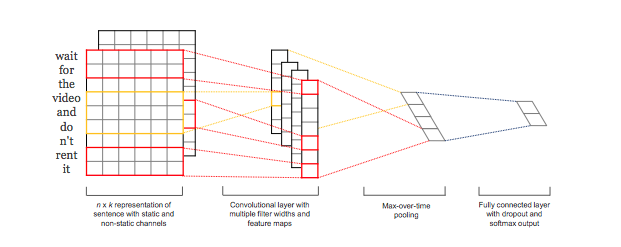
\includegraphics[scale=.7]{sentence-cnn.png}
\caption{Convolutional neural network for sentence classification obtained from \cite{kim2014convolutional}}
\label{fig:conv-sen}
\end{figure}
\subsubsection{Character level}
Recently it has also be shown that identifying sentences on the character level can increase performance. \citeA{zhang2015character} represented sentences as a matrix of one-hot-encoded character vectors with an alphabet size of 70 characters. Which was then used as input to a convolutional neural network. Since the input size of a convolutional neural network is fixed in size, smaller sentences where padded with only-zero vectors, together with characters that weren't in the alphabet. Using a convolutional neural network architecture similar to what is used in image recognition tasks, they classified a sentence. They generally performed better then word 2 vec based models. On smaller datagrams ngram based approaches would work better, only larger datasets they had the best performance. 
\todo[inline]{A lot of papers note that reversing the sentences increase performance of their task at hand, including these authors. I don't really understand why, but might be useful to note here.}

\section{For different tasks, same patterns will be valuable}
\subsection{Multi task neural networks}
One crucial aspect of this problem is that in order to determine the different attributes solving the same sub-tasks can help. To determine either calories or protein in your meal you probably have to understand the ingredients in the meal and the quantities. The cuisine can probably also be determined using the ingredients and might be helped by the quantities etc. 

 To simultaneously predict the pose and category in images  \citeA{elhoseiny2015convolutional} shared the same network for both tasks expects that near the end two branches where made: one for each task. They tried different positions of the branch split. 
\begin{figure}[h]
\centering
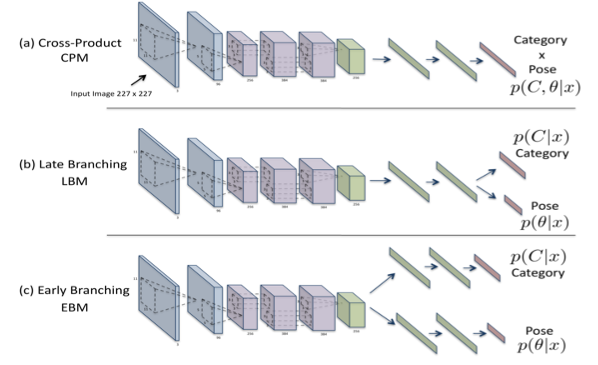
\includegraphics[scale=.5]{multitask.png}
\caption{A multi-objective convolutional neural network for pose and category estimation. Three architectures are shown with different branch split depths. Obtained from \cite{elhoseiny2015convolutional}}
\label{fig:mutliobj}
\end{figure}
If the errors would be $l_0$ and $l_1$ for the two tasks respectively they just define the loss function $\lambda_0 l_0 + \lambda_1 l_1$. for the complete network. They achieve state-of-the-art results for both tasks on two datasets. Similar approaches have been used to combine face verification(verifying that two faces are equal) and face identification(the location of the image) \cite{sun2014deep}. 
\todo[inline]{The work on face verification is actually highly related to what i proposed for food recognition, might be interesting. Wasn't able to find any multi-objective work for NLP }
\subsection{Transfer learning}
Another way of sharing your information is by re-using the weights of a network trained on one network and re-using it for another network. \citeA{collobert2008unified} for example re-used word embeddings. First they trained on a unsupervised language model task, next they trained on some other well known tasks(POS tagging followed by named entity recognition) while re-using the the word embeddings of the previous task, to eventually show some remarkable results on their final task semantic role labeling.

In general transfer learning can be really useful when you first train a network on a large dataset. Since for similar tasks the low level features learned will be the same, one can solve another task with a smaller dataset. By just re-training the last layers or fine-tuning all the layers \cite{erhan2010does}. 

This is often used for image recognition where the features learned with the large datasets in the image-net challenge\footnote{\url{http://www.image-net.org/}}. Given an smaller dataset on a different task these features can then be re-used by just replacing or/and retraining the last layers. 

We could do something similar if by predicting the recipe attribute our network was forced to learn low level features for our ingredient sentences. We could then create small data-sets that separate quantities from ingredient for example and train a model that those that by reusing our weights. 
\section{Proposal}
In my research I would like to train neural network(s) based on the schema.org dataset. For now I will only focus on the ingredient sentences as input, the instructions might be useful to predict preparation time but i will ignore it for now. The input of such a network would be a 3 dimensional matrix. The first dimension will contain the one-hot-encoded character vectors, the second dimension will describe all the characters of a ingredient sentence based on this one-hot-encoded vectors.  To account for different number of characters in the ingredient sentences I will pad the sentences to a fixed size with all-zero-vectors. Just like \cite{zhang2015character} did. The third dimension will then consist of the ingredient sentences representations in a recipe. Again to account for different number of ingredient sentences per ingredient I  will pad again to a fixed size will all-zero matrixes. 

\todo[inline]{A RNN architecture would require less padding, but based on the literature I belief that this should work very well. Even more so since ingredient sentences are not sequential  }

Next a set of convolutional layers will convert our textual input to higher level features. I propose to keep the third dimension in tact. Hence all convolutional layers only look at one recipe sentence at a time, and do consider them separately until  higher level layers. I belief this makes sense for the problem: you first have to understand the ingredient sentences before you can do something else. Secondly it also makes sure that our network is not able to over fit on certain orderings of ingredients. Thirdly these convolutional network per ingredient sentence could  also be used separately for some of the other tasks I proposed above. 

On top of these per ingredient sentence convolutional network we could then do two things:
\begin{itemize}
\item \textbf{Go directly to nutritional information per ingredient sentence}\\ Theoretically we could force the network to learn the nutritional information per ingredient sentence. For example the number of calories in this ingredient. By letting the network predict the nutritional information per ingredients sentence and then define the loss function based on the sum of these outputs: 
$$ (\sum_{n \in N}(\sum_{i \in I} y_n_i) - t_n)^2 $$
Where $N$ is the set of nutritional properties to predict and $I$ are the ingredient sentences in the recipe. $y_n_i$ is the predicted nutritional information $n$ for sentence ingredient $i$ and $t_n$ is the nutritional information of type $n$ for the complete recipe. Possibly we have to add a constraint to make sure ingredients can not have negative nutritional information. 

Please note that it might be a good idea to somehow constraint the loss function such that the networks can not output values below 0. 

\item \textbf{Combine information}\\ If we are not so much interested in the nutritional information per ingredient sentence we could also add a couple of layers that consider multiple ingredients at once (possibly fully connected or convolutional) to predict the nutritional information for the recipe network. This should allow the network to account for ingredient inter dependencies. For example a network might have a ingredient sentence "olive oil" without quantity estimation. If all other ingredients have quantities we might be able to estimate the amount of oil used. These ingredient sentence networks might also be more use able for other tasks described above. Since their output should contain more information.
\end{itemize}

I also want to make use of the multi-task/objective principle to predict the different attributes of a recipe(I already did this implicitly in the equation above) . However in this case some attributes will not be available and thus we have to somehow define a error function that can deal with this. We also have to see how we balance the errors different tasks. All recipes have a title however so we could always just try to predict the words in the title. A lot will depend on what our actual dataset looks like. 

Also I have to look at the exact network structure used: probably we can inspire this on existing NLP network. In general I belief my problem has a lot of similarities only that it could be a little simpler since the recipe/ingredient sentences are just a subset of all natural language possible. 

In the following weeks I would like to start to collect my dataset and based on that define my architecture in more detail. 

\bibliographystyle{apacite}
\bibliography{bib}
\section{Appendix}
\subsection{Interesting links}
This section shows some useful links and repositories that might be useful for later reference:
\begin{itemize}
\item \url{https://github.com/brandonmburroughs/RecipesScraper} scraper that can scrape allrecipes.com, jamieoliver, and epicurious.
\item \url{https://github.com/altosaar/food2vec/blob/master/src/csv\_to\_train\_file.sh} script used by food2vec to remove quantities. 
\end{itemize}
\end{document}
